% ---
\chapter{Conceitos, definições e resultados fundamentais em compressão de dados}
% ---
Este capítulo apresenta algumas definições, conceitos e resultados fundamentais para o entendimento das técnicas de compressão que serão discutidas em capítulos posteriores.

% -- Definições básicas de código
\section{Código}

Dado um conjunto $A$, usaremos a notação $A^+$ para definir o conjunto
que contém todas as cadeias não-vazias formadas pelas possíveis
combinações de $A$. Ou seja,
\begin{equation*}
  \emph{A}^+ = \Big\{
  (a_1,a_2,\dotsc, a_n) \colon n\in\mathbb{N}, \ n>0,
  \ a_i \in A \ \forall i \in \{1,\dotsc,n\} 
  \Big\}
\end{equation*}
Por simplicidade de notação, utilizaremos $a_1a_2\dotsm a_n$ para
denotar a sequência $(a_1,a_2,\dotsc, a_n)$ quando não houver
ambiguidade.

Um \textbf{alfabeto} $A$ é um conjunto finito. Chamaremos os elementos
de $A$ de \textbf{símbolos} ou \textbf{letras} e os elementos de $A^+$
de \textbf{cadeias} ou \textbf{palavras}.

Um \textbf{código} $C$ mapeia cada símbolo $m \in M$ para uma cadeia
em $W^+$. Mais precisamente, um código é uma função injetora de um
conjunto $M$ para $W^+$. O conjunto $M$ é chamado de \textbf{alfabeto
  de origem} e $W$ é chamado de\textbf{alfabeto código}. Chamaremos
cada cadeia na imagem de $C$ de \textbf{palavra-código}.

Dentro deste contexto, definimos o \textbf{comprimento} de uma palavra
$w\in W^+$, denotado por $l(w)$, como o inteiro positivo que
representa o tamanho da sequência $w$.

Tome como exemplo o alfabeto de origem $M = \{a, b, c\}$ e o alfabeto
código $W = \{0, 1\}$ composto somente por valores binários,
poderíamos definir um código $C$ da seguinte forma:

\begin{table}[!h]
   \centering
   \caption{Tabela do código C} \label{tab:vcode}
   \begin{tabular}{|l|c|c|c|c|c|c|r|}
        \hline
        \small{alfabeto de origem} & \small{palavra-código} \\ \hline
              a &   1   \\ \hline
              b &   01  \\ \hline
              c &   00  \\ \hline
  \end{tabular}
\end{table}
Neste exemplo, o \textbf{comprimento} da palavra-código associado à
letra ``b''~é dado por $l(C(b)) = l(01) = 2$.

As palavras-código associadas a cada símbolo podem ter um tamanho \emph{fixo} ou \emph{variável}.
Códigos nos quais palavras-código possuem um comprimento fixo são chamados de \textbf{códigos de comprimento fixo}, enquanto os que possuem alfabetos de comprimento variáveis são chamados \textbf{códigos de comprimento variável}. Note que o exemplo anterior é um código de comprimento variável. 
Provavelmente o exemplo mais conhecido de código de \textbf{comprimento fixo} seja código ASCII, que mapeia 64 símbolos alfa-numéricos (ou 256 em sua versão estendida) para palavras-código de 8 bits. 
Todavia, no contexto de compressão de dados procuramos construir códigos que podem variar em seu comprimento baseados na sua probabilidade associada, a fim de reduzir o tamanho médio da \emph{string} original ao codificá-la.

\subsection{Códigos unicamente decodificáveis e livres de prefixo}

%Um código é \textbf{distinto} se pode ser representado como uma função \textbf{bijetora}, i.e, $\forall$ $m_1$, $m_2$ $\in$ M, \emph{C($m_1$)} $\neq$ \emph{C($m_2$)}.
Um código é dito \textbf{unicamente decodificável} se qualquer palavra-código pode ser identificada quando imersa em uma sequência de palavras-código.

Um \textbf{código livre de prefixo} é um código unicamente decodificável em que nenhuma palavra-código é prefixo de outra. 
Por exemplo, o código que possuí sua imagem no conjunto de palavras-código \emph{$W^+$} := $\{1, 01, 000, 001\}$ não possui nenhuma cadeia que é prefixo de outra, portanto é considerado um \textbf{código livre de prefixo}.
Códigos livres de prefixo podem ser \emph{decodificados instantaneamente}, pois, ao processar uma cadeia de sequência de palavras-código podemos decodificar cada uma delas sem precisar verificar o início da seguinte.

Um código livre de prefixo em que \emph{W} := \{0, 1\} pode ser modelado por uma \textbf{arvore binária}. 
Imagine que cada mensagem $\emph{m} \in \emph{M}$ é uma folha. A palavra-código \emph{C(m)} é o caminho \emph{p} da raiz até a folha \emph{m}, de maneira em que, para cada nó percorrido concatenamos um bit a \emph{p} ("0" quando o nó está a esquerda e "1" quando está a direita), tal árvore é chamada \textbf{árvore do código livre de prefixo}. Tomando como exemplo o código representado pela Tabela~\ref{tab:vcode} (claramente um código livre de prefixo), podemos representá-lo por uma árvore livre de prefixo da seguinte forma:

\begin{figure}[h]
   \centering
   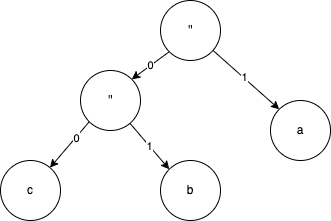
\includegraphics[scale=0.75]{figs/prefixtree.png}
    \caption{Árvore livre de prefixo}
    \label{fig:prefixt}
 \end{figure}
% ----------------------------------------------------------------------------
% Probabilidade -------------------------
\section{Relações fundamentais com a Teoria da Informação}
A codificação é comumente divida em duas componentes diferentes: \emph{modelo} e \emph{codificador}. 
O \emph{modelo} identifica a distribuição de probabilidade das mensagens baseado em sua semântica e estrutura. 
O \emph{codificador} toma vantagem de um possível \emph{bias} apontado pela modelagem, e utiliza as probabilidades associadas para reduzir a quantidade de dados necessária para representar a mesma informação (substituindo as mensagens que ocorrem com maior frequência por símbolos menores).
Isso significa que, a codificação está diretamente ligada as probabilidades associadas a cada mensagem.

Nesta seção, vamos construir o embasamento teórico necessário para entender a relação entre as probabilidades associadas e o comprimento das mensagens, e consequentemente criar uma noção dos parâmetros que devem ser maximizados para alcançar uma codificação eficiente.

\subsection{Distribuição de Probabilidade e Esperança}
Dado um experimento e um espaço amostral $\Omega$, uma \textbf{variável aleatória} \emph{X} associa um número real a cada um dos possíveis resultados em $\Omega$. Em outras palavras, \emph{X} é uma função que mapeia os elementos do espaço amostral para números reais. Uma variável aleatória é chamada \textbf{discreta} quando os valores dos experimentos associados a ela são números finitos ou ao menos infinitos que podem ser contados.
Podemos descrever melhor uma variável aleatória, atribuindo probabilidades sobre os valores que esta pode assumir. Esses valores são atribuídos pela \textbf{função de densidade de probabilidade}, denotada por \emph{$p_X$}. Portanto, a probabilidade do evento \{ \emph{X} = \emph{x} \} é a função de distribuição de probabilidade aplicada a x, \emph{i.e}, \emph{$p_X(x)$}.
\begin{equation} \label{eq:dist_prob_def}
p_X(x) = P(\{X = x\})
\end{equation}

Note que, a variável aleatória pode assumir qualquer um dos valores no espaço amostral que possuem uma probabilidade $\emph{P} > 0$, portanto
\begin{equation} \label{eq:dist_prob_sum}
\sum_{x ~\in ~im_X}^{}p_X(x) = 1.
\end{equation}

O \textbf{valor esperado} (ou \textbf{esperança}) da variável aleatória \emph{X} é definido como
\begin{equation} \label{eq:exp_val}
\textbf{E}[X] = \sum_{x ~\in ~im_X}^{} xp_X(x).
\end{equation}
%--------------------------------------
% ------------------------------ Entropia
\subsection{Comprimento médio do código}
Seja \emph{p} a distribuição de probabilidade associada ao alfabeto de origem \emph{M}. Assuma que \emph{C} é um código tal que \emph{C(m)} = \emph{w}, definimos o \textbf{tamanho médio} de \emph{C} como:
\begin{equation} \label{eq:code_len}
l_a (C) = \sum_{m \in M}^{} p(m) l(C(m))
\end{equation}

Um código \emph{C} unicamente decodificável é \textbf{ótimo} se $l_a(C)$ é mínimo, isto é, para qualquer código unicamente decodificável \emph{C'} temos que:
\begin{equation} \label{eq:code_len_optimal}
l_a(C) \leq l_a(C')
\end{equation}

\subsection{Entropia}
A \textbf{entropia de Shannon} aplica as noções de entropia física (que representa a aleatoriedade de um sistema) à Teoria da Informação. Dado um espaço de probabilidade \emph{X} e a função \emph{p} sendo a distribuição de probabilidade associada a \emph{X}, definimos \textbf{entropia} como:
\begin{equation} \label{eq:entropy}
H(X, p) = \sum_{x \in X}^{} p(x) \log_2 \frac{1}{p(x)}
\end{equation}

Por esta definição temos que quanto menor o \emph{bias} da função de distribuição de probabilidade relacionada ao sistema, maior a sua entropia. Em outras palavras, a entropia de um sistema esta intimamente ligada a sua  "desordem". 

Shannon (incluir referencia papper do Shannon) aplica o mesmo conceito de entropia no contexto da Teoria da Informação, "substituindo" o conjunto de estados \emph{S} pelo conjunto de mensagem \emph{M}, isto é, \emph{M} é interpretado como um conjunto de possíveis mensagens, tendo como \emph{p(m)} a probabilidade de $m \in M$.
Baseado na mesma premissa, Shannon mede a informação contida em uma mensagem da seguinte forma:
\begin{equation} \label{label:info_quantity}
\emph{i(m)} = \log_2 \frac{1}{p(m)}.
\end{equation}

\subsection{Comprimento de Código e Entropia}
Nas seções anteriores, o comprimento médio de um código  foi definido em função da distribuição de probabilidade associada ao seu alfabeto de origem.
Da mesma forma, as noções de \textbf{entropia} relacionada a um conjunto de mensagens, têm ligação direta com as probabilidades associadas a estas. 
A seguir, será mostrado como podemos relacionar o comprimento médio de um código a sua entropia através da \textbf{Desigualdade de Kraft-McMillan} , e por consequência estabelecer uma relação direta entre \textbf{a entropia de um conjunto de mensagens e a otimalidade do código associada a estas mensagens}.

\begin{lemma}[Desigualdade de Kraft-McMillan] 
\textbf{Kraft.}. Para qualquer conjunto \emph{L} de comprimento códigos que satisfaça:
\begin{align*}
\sum_{l \in L}^{} 2^{-l} \leq 1.
\end{align*}
Existe ao menos um código livre de prefixo tal que, $|w_i|$ = $l_i$ ~,~$\forall w \in W^+$.

\textbf{Kraft-McMillan.} Para todo código binário unicamente decodificável \textbf{\emph{C} : $\emph{M} \rightarrow \emph{W}^+$} .
\begin{equation*}
\sum_{w \in W^+}^{}2^{-l(w)} \leq 1.
\end{equation*}


\begin{proof}

\item \textbf{Desigualdade de Kraft}
Sem perda de generalidade, suponha que os elementos de \emph{L} estão ordenados de maneira em que:
\begin{align*}
l_1 \leq l_2 \leq ... \leq l_n
\end{align*}
Agora vamos construir um código livre de prefixo em uma ordem crescente de tamanho, de maneira em que $l(w_i) = l_i$. Sabemos que um código é livre de prefixo se e somente se ,existe uma palavra-código $w_j$  tal que nenhuma das palavras-código anteriores $(w_1, w_2, w_{j-1})$ são prefixo de $w_j$.

Sem as restrições de prefixo, uma palavra-código de tamanho $l_j$ poderia ser construída de $2^{l_j}$ maneiras diferentes. Com a restrição apresentada anteriormente, considerando uma palavra $w_k$ anterior a $w_j$ (i.e, $k < j$), existem $2^{l_j - l_k}$ possíveis palavras-código em que $w_k$ seria um prefixo, e que portanto não podem pertencer ao código. Chamaremos tal conjunto de "palavras-código proibidas". Vale notar que os elementos do conjunto de palavras-código proibidas são excludentes entre si, pois se duas palavras-código menores que \emph{j} fossem prefixo da mesma palavra-código, elas seriam prefixos entre si. 

Dito isto, podemos definir o tamanho do conjunto de palavras-código proibida para $w_j$.
\begin{equation*}
\sum_{i=1}^{j-1} 2^{l_j - l_i}
\end{equation*}

A construção do código livre de prefixo é possível se e somente se, existir ao menos uma palavra-código de tamanho $j > 1$ que não está contida no conjunto das palavras-código proibidas.
\begin{equation*}
2^{l_j} > \sum_{i=1}^{j-1} 2^{l_j - l_i}
\end{equation*}

Como o domínio do problema apresentado está restrito aos inteiros não negativos, podemos afirmar que:
\begin{align*}
2^{l_j} > \sum_{i=1}^{j-1} 2^{l_j - l_i} &= 2^{l_j} \geq \sum_{i=1}^{j-1} 2^{l_j - l_i} + 1 \\
&= 2^{l_j} \geq \sum_{i=1}^{j} 2^{l_j - l_i} \\
&= 1 \geq \sum_{i=1}^{j} 2^{-l_i} \\
&=  \sum_{i=1}^{j} 2^{-l_i} \leq 1
\end{align*}

Substituindo \emph{n} em \emph{j}, chegamos a desigualdade de Kraft.
\begin{equation*}
\sum_{l \in L}^{} 2^{-l} \leq 1.
\end{equation*}

Note que os argumentos utilizados para a construção da prova possuem dupla-equivalência, portando concluem a prova nos dois sentidos.

\item \textbf{Kraft-McMillan}
Suponha um código \textbf{unicamente decodificável} \emph{C} qualquer, e faça $l_{max}$ = $\max_{w}l(w)$.

Agora considere uma sequência de \emph{k} palavras-código de \textbf{\emph{C} : $\emph{M} \rightarrow \emph{W}^+$} (onde \emph{k} é um inteiro positivo). Observe que:

\begin{align*}
(\sum_{w \in W^+}^{}2^{-l(w)})^k &= (\sum_{w_1}^{}2^{-l(w_1)}) \cdot (\sum_{w_2}^{}2^{-l(w_2)}) \cdot ... \cdot (\sum_{w_k}^{}2^{-l(w_k)}) \\
&= \sum_{w_1}^{} \sum_{w_2}^{} ... \sum_{w_k}^{} \prod_{j = 1}^{k} 2^{-l(w_j)} \\
&= \sum_{w_1,..., w_k}^{} 2^{- \sum_{j=1}^{k} l(w_j)} \\
&= \sum_{w_k}^{} 2^{-l(w^k)} \\
&= \sum_{j=1}^{k \cdot l_{max}} |\{w_k | l(w_k) = j\}| \cdot 2^{-j}.
\end{align*}

Sabemos que existem $2^{j}$ palavras-código de tamanho \emph{j}, isto é, $|\{w_k | l(w_k) = j\}| = 2^j$. Para que o código seja unicamente decodificável obtemos o seguinte limite superior:
\begin{equation*}
(\sum_{w \in W^+}^{}2^{-l(w)})^k \leq \sum_{j=1}^{k \cdot l_{max}} 2^j \cdot 2^{-j} = k \cdot l_{max}
\end{equation*}

Logo,
\begin{equation*}
\sum_{w \in W^+}^{}2^{-l(w)} \leq (k \cdot l_{max})^ \frac{1}{k}
\end{equation*}

Note que a desigualdade é valida para qualquer $k > 0$ inteiro. Aproximando \emph{k} ao infinito, obtemos a desigualdade de Kraft-McMillan.

\begin{equation*}
\sum_{w \in W^+}^{}2^{-l(w)} \leq \lim_{k\to\infty} (k \cdot l_{max})^ \frac{1}{k} = 1.
\end{equation*}

\end{proof}
\end{lemma}

\begin{lemma}[Entropia como limite inferior para o comprimento médio] Dado um conjunto de mensagens \emph{M} associado a uma distribuição de probabilidades \emph{p} e um código unicamente decodificável \emph{C}.
\begin{equation*}
H(M, p) \leq l_a(C)
\end{equation*}

\begin{proof}
Queremos provar que $H(M, p) - l_a(C) \leq 0$, dado que  $H(M, p) \leq l_a(C) \Leftrightarrow H(M, p) - l_a(C) \leq 0$.

Substituindo a equação~\ref{eq:entropy} em \emph{H(M, p)} e~\ref{eq:code_len} em \emph{$l_a(C)$}, temos:

\begin{align*}
H(M, p) - l_a(C) &= \sum_{m \in M}^{}p(s) \log_2 \frac{1}{p(m)}  - \sum_{m \in M, w \in W^+}^{}p(m) l(w) \\
&= \sum_{m \in M, w \in W^+}^{}p(m) \left(  \log_2 \frac{1}{p(m)} - l(w) \right) \\
&= \sum_{m \in M, w \in W^+}^{}p(m) \left(  \log_2 \frac{1}{p(m)} - \log_2 2^{l(w)} \right) \\
&= \sum_{m \in M, w \in W^+}^{}p(m) \log_2 \frac{2^{-l(w)}}{p(m)}
\end{align*}

A \textbf{Desigualdade de Jansen} afirma que se uma função \emph{f(x)} é côncava, então $\sum_{i}{}p_i~f(x_i) \leq f(\sum_{i}{}p_i~x_i)$. Como a função $\log_2$ é côncava, podemos aplicar a Desigualdade de Jansen ao resultado obtido anteriormente.

\begin{equation*}
\sum_{m \in M, w \in W^+}^{}p(m) \log_2 \frac{2^{-l(w)}}{p(m)}  \leq \log_2(\sum_{m \in M, w \in W^+}{}2^{-l(w)})
\end{equation*}

Agora aplicamos a desigualdade de Kraft-McMillan, e concluímos que:

\begin{equation*}
H(M, p) - l_a(C) \leq \log_2(\sum_{m \in M, w \in W^+}{}2^{-l(w)}) \Rightarrow H(M, p) - l_a(C) \leq 0.
\end{equation*}


\end{proof}

\end{lemma}

\begin{lemma}[Entropia como limite superior para o comprimento médio de um código livre de prefixo ótimo] Dado um conjunto de mensagens \emph{M} associado a uma distribuição de probabilidades \emph{p} e um código livre de prefixo ótimo \emph{C}.
\begin{equation*}
l_a(C) \leq H(M, p) + 1
\end{equation*}

\begin{proof}
Sem perda de generalidade, para cada mensagem $m \in M$ faça \emph{l(m)} = $\left \lceil{\log_2 \frac{1}{p(m)} }\right \rceil $. Temos que:
\begin{align*}
\sum_{m \in M}^{} 2^{-l(m)} &= \sum_{m \in M}^{} 2^{-\left \lceil{\log_2 \frac{1}{p(m)} }\right \rceil} \\
&\leq \sum_{m \in M}^{} 2^{-{\log_2 \frac{1}{p(m)} }} \\
&= \sum_{m \in M}^{} p(m) \\
&= 1
\end{align*}

De acordo com a desigualdade de Kraft-McMillan existe um código livre de prefixo \emph{C'}  com palavras-código de tamanho \emph{l(m)}, portanto:
\begin{align*}
l_a(C') &=  \sum_{m \in M', w \in W'^+}^{}p(m) l(w) \\
&=  \sum_{m \in M', w \in W'^+}^{}p(m) \left \lceil{\log_2 \frac{1}{p(m)} }\right \rceil \\
&\leq \sum_{m \in M', w \in W'^+}^{}p(m) (1 + \log_2 \frac{1}{p(m)}) \\
&= 1 +  \sum_{m \in M', w \in W'^+}^{}p(m) \log_2 \frac{1}{p(m)} \\
&= 1 + H(M)
\end{align*}

Pela definição de código livre de prefixo ótimo, $l_a(C) \leq l_a(C')$, isto é:
\begin{equation*}
l_a(C) \leq H(M, p) + 1 
\end{equation*}
\end{proof}
\end{lemma}


% ------------------- End of chapter 1 -----------------------------

% --- Guardando para exemplo
% A formatação das referências bibliográficas conforme as regras da ABNT são um
% dos principais objetivos do \abnTeX. Consulte os manuais
% \citeonline{abntex2cite} e \citeonline{abntex2cite-alf} para obter informações
% sobre como utilizar as referências bibliográficas.

% %-
% \subsection{Acentuação de referências bibliográficas}
% %-

% Normalmente não há problemas em usar caracteres acentuados em arquivos
% bibliográficos (\texttt{*.bib}). Na~\autoref{tabela-acentos} você encontra alguns exemplos das conversões mais importantes. Preste atenção especial para `ç' e `í'
% que devem estar envoltos em chaves. A regra geral é sempre usar a acentuação
% neste modo quando houver conversão para letras maiúsculas.

% \begin{table}[htbp]
% \caption{Tabela de conversão de acentuação.}
% \label{tabela-acentos}

% \begin{center}
% \begin{tabular}{ll}\hline\hline
% acento & \textsf{bibtex}\\
% à á ã & \verb+\`a+ \verb+\'a+ \verb+\~a+\\
% í & \verb+{\'\i}+\\
% ç & \verb+{\c c}+\\
% \hline\hline
% \end{tabular}
% \end{center}
% \end{table}


% ---
% \section{Deu pau em algo?}
% ---

% Consulte a FAQ com perguntas frequentes e comuns no portal do \abnTeX:
% \url{https://code.google.com/p/abntex2/wiki/FAQ}.

% Inscreva-se no grupo de usuários \LaTeX:
% \url{http://groups.google.com/group/latex-br}, tire suas dúvidas e ajude a galera se tiver tudo certo.


